\chapter{Marco teórico y estado del arte}
\label{chap:marco-teorico}

\section{Software como dispositivo médico (SaMD)}
\label{sec:samd}

El uso de \textit{software} en el ámbito de la salud comprende aplicaciones
con diferentes finalidades, desde funciones administrativas hasta sistemas
destinados a proporcionar información utilizada con propósitos médicos.
Dentro de este contexto surge el concepto de \textit{Software as a Medical
Device} (SaMD), utilizado para distinguir determinadas funciones de
\textit{software} que cumplen por sí mismas una finalidad médica de aquellas
que forman parte del \textit{hardware} de un dispositivo médico.

\subsection{Concepto y características de SaMD}
\label{subsec:concepto-samd}


El \textit{International Medical Device Regulators Forum} (IMDRF) define el
\textit{software} como dispositivo médico como aquel \textit{software}
destinado a ser utilizado para uno o más propósitos médicos que cumplen
dichos propósitos sin formar parte del \textit{hardware} de un dispositivo
médico \citep{IMDRF2013SaMD}. Esta definición permite diferenciar el SaMD
del \textit{software} incorporado o integrado físicamente como parte de un
dispositivo médico.

Una característica relevante del SaMD es que puede ejecutarse en plataformas
informáticas de propósito general y no requiere formar parte del
\textit{hardware} de un dispositivo médico para cumplir su finalidad.
Asimismo, puede interactuar con otros productos, incluidos dispositivos
médicos y otros sistemas de \textit{software}, mediante diferentes
mecanismos de comunicación e intercambio de información
\citep{IMDRF2013SaMD}.

La consideración de un \textit{software} dentro de esta categoría depende
de su finalidad prevista y de las funciones que desempeña en el contexto
médico. Por este motivo, no todo \textit{software} utilizado dentro de una
institución de salud constituye necesariamente un SaMD. Las aplicaciones
destinadas exclusivamente a funciones administrativas o de gestión, por
ejemplo, se diferencian de aquellas cuyas funciones están destinadas a
cumplir un propósito médico.

El IMDRF ha desarrollado además un marco específico para abordar aspectos
relacionados con la categorización de riesgo, los sistemas de gestión de
calidad y la evaluación clínica del SaMD. Estos documentos consideran, entre
otros aspectos, la importancia de la información proporcionada por el \textit{software} para la toma de decisiones relacionadas con la atención sanitaria y la situación o condición clínica en la que dicha información es utilizada \citep{IMDRF2014SaMDRisk}.

\subsection{Software de apoyo al diagnóstico clínico}
\label{subsec:software-apoyo-diagnostico}

El \textit{software} de apoyo a la toma de decisiones clínicas comprende funciones
destinadas a proporcionar a los profesionales de la salud información que
pueda ser utilizada durante la evaluación de un paciente. Estas herramientas
pueden organizar, relacionar o presentar información clínica con el propósito
de complementar el análisis realizado por el profesional, sin que ello
implique necesariamente la sustitución de su criterio durante la toma de
decisiones \citep{FDA2026CDS}.

Dentro del ámbito del \textit{Clinical Decision Support} (CDS), la
\textit{U.S. Food and Drug Administration} (FDA) establece criterios para
diferenciar determinadas funciones de \textit{software} destinadas a apoyar
a los profesionales de aquellas que pueden encontrarse sujetas a la
regulación aplicable a dispositivos médicos. Entre los aspectos
considerados se encuentran el tipo de información procesada, la
naturaleza de la salida proporcionada por el \textit{software} y la
posibilidad de que el profesional revise de manera independiente el
fundamento de las recomendaciones presentadas \citep{FDA2026CDS}.

En este contexto, existe una diferencia entre proporcionar información u
opciones que complementen la evaluación del profesional y generar una salida
específica destinada a prevenir, diagnosticar o tratar una enfermedad. La FDA
considera además relevante que determinadas funciones de apoyo no estén
destinadas a reemplazar o dirigir el juicio del profesional y que este pueda
comprender y revisar la base de la información o recomendación proporcionada
antes de utilizarla en una decisión clínica \citep{FDA2026CDS}.

El tratamiento de señales médicas requiere consideraciones particulares.
La FDA distingue las funciones de \textit{software} destinadas a adquirir,
procesar o analizar señales provenientes de sistemas de adquisición de
aquellas funciones que se limitan a presentar o relacionar información
médica. Esta distinción resulta relevante para sistemas que incorporan el
procesamiento computacional de señales fisiológicas, debido a que las
características de la información de entrada y la finalidad prevista de
los resultados forman parte de los aspectos considerados al determinar
la naturaleza de la función del \textit{software}
\citep{FDA2026CDS}.


En sistemas que incorporan técnicas de inteligencia artificial, los resultados
del procesamiento pueden utilizarse como información complementaria para
orientar la atención del profesional hacia determinados elementos del
registro. Sin embargo, la utilización de estos resultados como apoyo requiere
mantener claramente diferenciadas la salida generada por el sistema y la
interpretación clínica realizada por el profesional, especialmente cuando
la información analizada puede intervenir en procesos relacionados con el
diagnóstico.

En las herramientas de apoyo a la revisión electroencefalográfica, la
información obtenida mediante procesamiento automatizado debe presentarse
como un elemento complementario a la interpretación clínica. La valoración
de las señales EEG y la determinación de su relevancia diagnóstica
permanecen bajo responsabilidad del profesional especialista.



\section{Epilepsia}
\label{sec:epilepsia}

La epilepsia es una enfermedad cerebral crónica no transmisible que puede
afectar a personas de todas las edades y constituye una de las enfermedades
neurológicas más frecuentes a nivel mundial. Se estima que aproximadamente
50 millones de personas viven con epilepsia, con una proporción importante
de los casos concentrada en países de ingresos bajos y medianos
\citep{WHO2024Epilepsy}.

Una crisis epiléptica corresponde a una manifestación transitoria producida
por una actividad neuronal cerebral anormal, excesiva o sincrónica. Sus
manifestaciones pueden variar considerablemente según las regiones cerebrales
involucradas y pueden incluir alteraciones del movimiento, la sensibilidad,
la conciencia y otras funciones cognitivas. Por este motivo, las crisis
epilépticas no se manifiestan exclusivamente mediante episodios convulsivos,
sino que pueden presentarse de diferentes formas y con distinta duración e
intensidad \citep{Fisher2014EpilepsyDefinition,WHO2024Epilepsy}.

La presencia de una única crisis no implica necesariamente el diagnóstico de
epilepsia. La \textit{International League Against Epilepsy} (ILAE) establece una
definición clínica operacional según la cual la epilepsia puede considerarse
presente cuando ocurren al menos dos crisis no provocadas o reflejas separadas
por más de 24 horas; cuando ocurre una crisis no provocada o refleja y existe
una probabilidad de nuevas crisis similar al riesgo general de recurrencia
después de dos crisis no provocadas, de al menos 60\% durante los siguientes
10 años; o cuando se diagnostica un síndrome epiléptico
\citep{Fisher2014EpilepsyDefinition}. Esta definición permite contemplar
diferentes situaciones clínicas y resalta que el diagnóstico no depende
únicamente del número de crisis observadas.

Las causas de la epilepsia son diversas. La Organización Mundial de la Salud
señala categorías etiológicas estructurales, genéticas, infecciosas,
metabólicas, inmunológicas y desconocidas. Entre las condiciones que pueden
estar relacionadas con su aparición se encuentran determinadas lesiones
cerebrales, alteraciones congénitas o genéticas, traumatismos
craneoencefálicos, accidentes cerebrovasculares, infecciones del sistema
nervioso y tumores cerebrales. No obstante, en una proporción importante de
los casos la causa puede permanecer desconocida \citep{WHO2024Epilepsy}.

La diversidad de las manifestaciones clínicas y de los mecanismos asociados
con la epilepsia hace necesario recurrir a diferentes elementos durante su
evaluación. Entre ellos se encuentran los antecedentes y la historia clínica
del paciente, las características observadas durante las crisis y los
resultados de estudios complementarios. Dentro de estos últimos, el
electroencefalograma desempeña un papel relevante al permitir registrar y
examinar la actividad eléctrica cerebral y aportar información útil para la
evaluación de pacientes con sospecha o diagnóstico de epilepsia
\citep{NoachtarRemi2009}.

La relación entre epilepsia y actividad eléctrica cerebral fundamenta
la utilización de estudios electroencefalográficos en la evaluación clínica.
Por ello, resulta necesario comprender los principios de la
electroencefalografía y las características de las señales EEG, aspectos
que se desarrollan en la siguiente sección.



\section{Electroencefalografía}
\label{sec:electroencefalografia}

La electroencefalografía es una técnica utilizada para registrar y examinar
la actividad eléctrica cerebral mediante señales obtenidas a través de
electrodos. El registro resultante, denominado electroencefalograma (EEG),
permite observar variaciones de la actividad eléctrica cerebral a lo largo
del tiempo y constituye una herramienta ampliamente utilizada en el ámbito
de la neurología clínica \citep{StLouisFrey2016EEG}.

\subsection{Electroencefalograma (EEG)}
\label{subsec:electroencefalograma}

El electroencefalograma es el registro de las variaciones de potencial
eléctrico obtenidas mediante electrodos colocados sobre el cuero cabelludo.
Estas variaciones se encuentran relacionadas principalmente con la actividad
eléctrica generada por poblaciones de neuronas cerebrales y, luego de su
adquisición y amplificación, pueden representarse como señales que varían en
función del tiempo \citep{StLouisFrey2016EEG}.

El EEG constituye un procedimiento no invasivo que permite estudiar la
actividad cerebral con una elevada resolución temporal. Durante un registro
pueden observarse patrones fisiológicos relacionados, entre otros factores,
con el estado de vigilia, el sueño y determinadas condiciones del paciente,
así como alteraciones que pueden resultar relevantes para la evaluación
neurológica. La interpretación del registro requiere considerar tanto las
características de las formas de onda como el contexto clínico en el que
estas se presentan \citep{StLouisFrey2016EEG}.

En el estudio de la epilepsia, el EEG desempeña un papel particularmente
importante debido a que puede aportar información que apoye el diagnóstico
y la clasificación de las epilepsias. Durante una crisis pueden registrarse
patrones electroencefalográficos ictales, mientras que entre las crisis
pueden observarse determinadas descargas epileptiformes interictales. No
obstante, los hallazgos electroencefalográficos deben interpretarse en
conjunto con la información clínica y no de manera aislada
\citep{NoachtarRemi2009,StLouisFrey2016EEG}.

El registro electroencefalográfico se obtiene de manera simultánea desde
diferentes ubicaciones del cuero cabelludo. La disposición de los electrodos
y la forma en que sus señales son combinadas permiten representar la
actividad registrada desde distintas regiones y analizar su distribución
espacial y temporal. Para favorecer la reproducibilidad de los registros se
emplean sistemas estandarizados de posicionamiento de electrodos y diferentes
configuraciones de visualización denominadas montajes
\citep{StLouisFrey2016EEG}.

En los sistemas digitales, las señales adquiridas pueden almacenarse para su
posterior visualización y análisis mediante herramientas informáticas. Esto
permite modificar parámetros de presentación, recorrer diferentes intervalos
temporales del registro y aplicar configuraciones que faciliten la inspección
de las señales sin alterar el registro original almacenado. Estas características son especialmente relevantes en registros EEG de
larga duración, en los que el profesional necesita examinar diferentes
canales e intervalos temporales del estudio
\citep{StLouisFrey2016EEG}.


La revisión digital de registros EEG requiere herramientas que permitan
representar los canales y explorar distintos períodos del estudio. Para
comprender estas representaciones, es necesario analizar cómo se organizan
las señales y los canales que conforman un registro EEG.



\subsection{Señales y canales EEG}
\label{subsec:senales-canales-eeg}

Las señales EEG representan variaciones de potencial eléctrico registradas a
lo largo del tiempo mediante electrodos ubicados en diferentes posiciones del
cuero cabelludo. En una representación convencional del EEG, el eje horizontal
corresponde al tiempo y el eje vertical representa las variaciones de voltaje
registradas. Debido a la pequeña amplitud de las señales obtenidas en el cuero
cabelludo, estas suelen expresarse en microvoltios ($\mu$V)
\citep{StLouisFrey2016EEG}.

El registro electroencefalográfico se basa en la medición de diferencias de
potencial eléctrico.  Por este motivo, un canal EEG no corresponde a la medición aislada de un electrodo, sino a la diferencia de potencial eléctrico
registrada entre dos entradas de un amplificador diferencial. De esta manera, cada canal o derivación representa la diferencia de potencial entre dos puntos
de registro, que pueden corresponder a dos electrodos ubicados sobre el cuero
cabelludo o a un electrodo y una referencia definida para el registro
\citep{StLouisFrey2016EEG}.

Si se consideran dos entradas de un canal, convencionalmente denominadas
G1 y G2, la señal representada corresponde a la diferencia de potencial entre
ambas. Las variaciones relativas entre estas entradas determinan la dirección
de las deflexiones observadas en el trazado. Por convención, cuando G1 es más
negativo que G2, la deflexión se representa hacia arriba, mientras que la
situación opuesta produce una deflexión hacia abajo. Esta convención permite
comparar la polaridad de las formas de onda entre diferentes canales y
contribuye a la localización de la actividad registrada
\citep{StLouisFrey2016EEG}.

Un registro EEG está compuesto por múltiples canales observados de manera
simultánea. Cada uno proporciona información sobre diferencias de potencial
correspondientes a determinadas ubicaciones, mientras que su análisis conjunto
permite examinar la distribución espacial y temporal de la actividad
registrada. La comparación entre canales resulta particularmente importante
para identificar diferencias entre regiones, reconocer patrones y determinar
en qué zonas determinadas formas de onda presentan mayor expresión
\citep{StLouisFrey2016EEG}.

La amplitud de las formas de onda constituye una de las características
utilizadas durante la inspección del EEG. En los sistemas digitales, la sensibilidad de visualización puede ajustarse para modificar la escala vertical con la que se representan las señales en pantalla. Este ajuste afecta la representación visual de las formas de onda y permite facilitar su inspección, pero no modifica los valores originales de la señal almacenada
\citep{StLouisFrey2016EEG}.

La forma en que los electrodos son seleccionados y relacionados para construir
los distintos canales determina la configuración utilizada para presentar el
EEG. Por este motivo, la interpretación de un registro requiere conocer tanto
la ubicación de los electrodos como las relaciones establecidas entre ellos.
Los sistemas estandarizados de posicionamiento permiten identificar de manera
consistente las regiones desde las cuales se obtienen las señales y sirven de
base para la construcción de los diferentes montajes utilizados durante la
revisión electroencefalográfica \citep{StLouisFrey2016EEG}.


\subsection{Sistema internacional 10-20 y mapa de electrodos}
\label{subsec:sistema-10-20}

Para obtener registros electroencefalográficos comparables y reproducibles
es necesario utilizar criterios estandarizados para la ubicación de los
electrodos sobre el cuero cabelludo. Uno de los sistemas empleados para este
propósito es el Sistema Internacional 10-20, utilizado como referencia para
el posicionamiento de electrodos en registros EEG clínicos
\citep{Acharya2016ElectrodeNomenclature}.

El nombre 10-20 se relaciona con las proporciones utilizadas para determinar
las posiciones de los electrodos. Estas se establecen a partir de mediciones realizadas entre puntos anatómicos de referencia de la cabeza, principalmente el nasion, ubicado en la unión entre la frente y la raíz de la nariz; el inion,
correspondiente a la prominencia ósea posterior del cráneo; y los
puntos preauriculares, situados delante de las orejas. Sobre las líneas obtenidas
mediante estas mediciones, las posiciones se determinan utilizando intervalos
correspondientes al 10\% o al 20\% de las distancias medidas. El empleo de
proporciones permite adaptar la distribución de los electrodos a las
dimensiones de la cabeza de cada paciente manteniendo posiciones relativas
comparables \citep{StLouisFrey2016EEG,Acharya2016ElectrodeNomenclature}.

Cada posición se identifica mediante una combinación de letras y números.
Las letras hacen referencia a regiones de la cabeza asociadas con las áreas
cerebrales subyacentes: Fp corresponde a la región frontopolar, F a la
frontal, C a la central, P a la parietal, T a la temporal y O a la occipital.
La letra ``z'', asociada al término inglés \textit{zero}, identifica las posiciones situadas sobre la línea media. Los números impares se utilizan para posiciones del hemisferio izquierdo y los números pares para las correspondientes al hemisferio derecho \citep{StLouisFrey2016EEG,Acharya2016ElectrodeNomenclature}.

Esta nomenclatura permite identificar de manera sistemática la procedencia
espacial de las señales registradas. Por ejemplo, denominaciones como Fp1,
F3, C3, P3 y O1 corresponden a posiciones del lado izquierdo, mientras que
Fp2, F4, C4, P4 y O2 identifican posiciones correspondientes del lado
derecho. Posiciones como Fz, Cz y Pz se encuentran sobre la línea media.
La organización espacial de estos puntos puede representarse mediante un
mapa de electrodos, como se muestra en la Figura~\ref{fig:sistema-10-20}.

\begin{figure}[H]
    \centering
    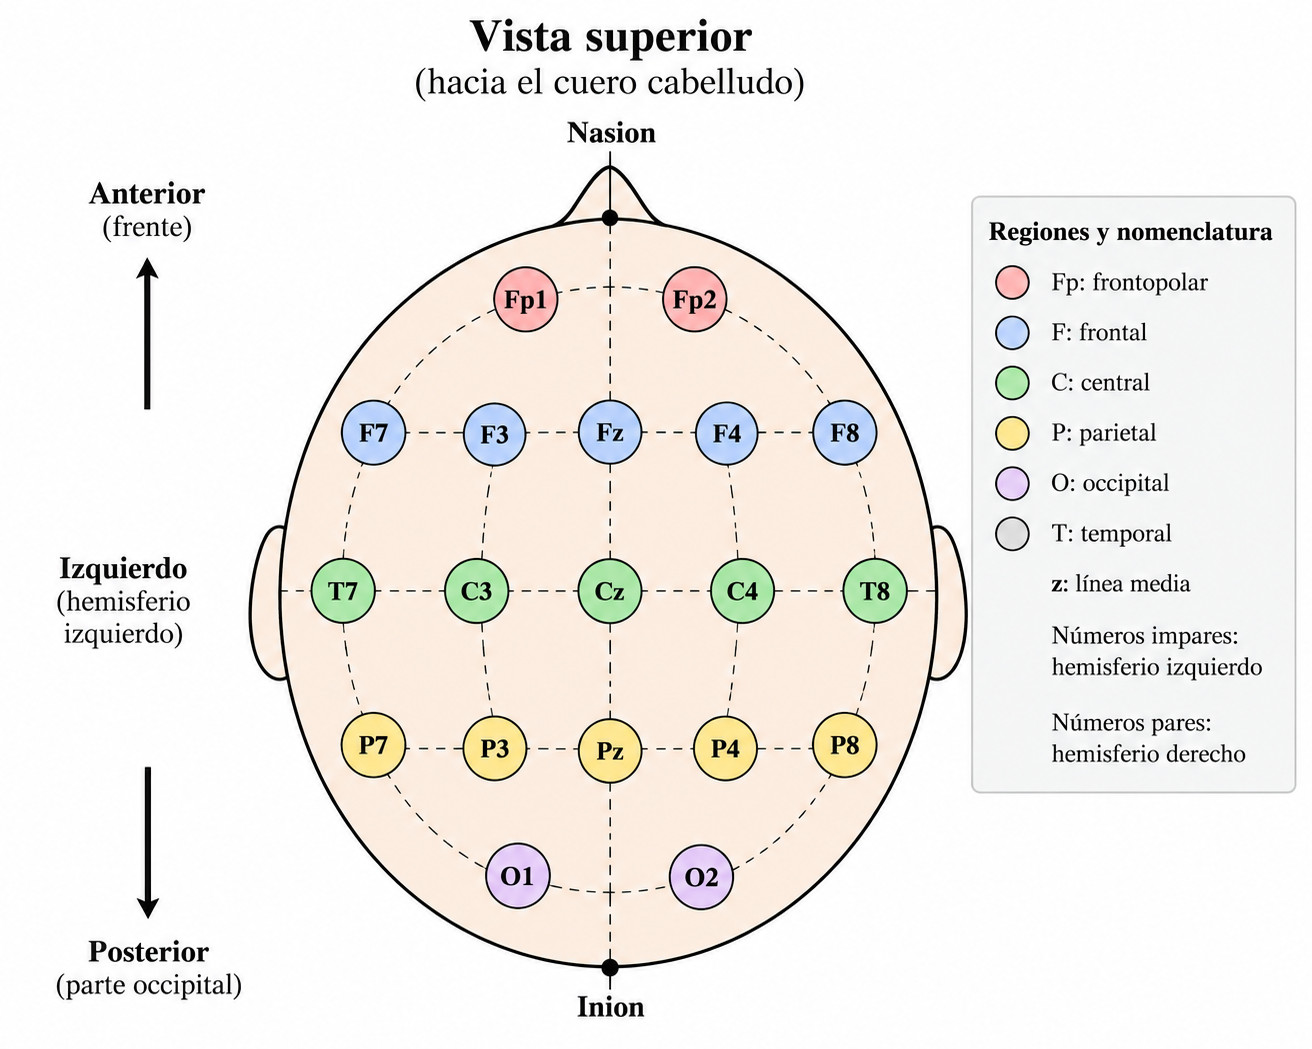
\includegraphics[width=0.90\textwidth]{ThesisFigs/sistema_10_20.png}
    \caption{Distribución de electrodos según el Sistema Internacional 10-20.
    Elaboración propia basada en \citet{StLouisFrey2016EEG} y
    \citet{Acharya2016ElectrodeNomenclature}.}
    \label{fig:sistema-10-20}
\end{figure}

La utilización de posiciones estandarizadas facilita la comparación de la
actividad registrada entre diferentes regiones y proporciona una referencia
común para la construcción de los canales EEG. Asimismo, permite establecer
configuraciones reproducibles para la presentación de las señales durante
su revisión. A partir de las relaciones establecidas entre estos electrodos
se construyen diferentes montajes electroencefalográficos, los cuales se
desarrollan en la siguiente subsección
\citep{Acharya2016ElectrodeNomenclature}.


\subsection{Montajes electroencefalográficos}
\label{subsec:montajes-eeg}

Un montaje electroencefalográfico corresponde a la organización de los
canales utilizados para presentar simultáneamente las señales de un registro
EEG. A partir de un mismo conjunto de electrodos pueden establecerse
diferentes relaciones entre sus señales, permitiendo visualizar la actividad
eléctrica cerebral desde distintas configuraciones sin modificar el registro
original. La selección del montaje constituye, por tanto, un elemento
importante durante la revisión e interpretación del EEG
\citep{StLouisFrey2016EEG,Acharya2016Montages}.

Los montajes pueden organizarse principalmente en configuraciones bipolares
y referenciales. En un montaje bipolar, cada canal representa la diferencia
de potencial entre dos electrodos del cuero cabelludo y los electrodos
adyacentes pueden disponerse formando secuencias o cadenas. En este tipo de
representación, un mismo electrodo puede participar en canales consecutivos,
lo que permite comparar la actividad entre regiones vecinas y contribuir a
la localización de determinadas formas de onda
\citep{Acharya2016Montages}.

Una configuración ampliamente utilizada es el montaje bipolar longitudinal,
en el cual los electrodos se relacionan siguiendo cadenas orientadas
principalmente en sentido anteroposterior. Este tipo de montaje es conocido
también de manera habitual como montaje de ``doble banana'', debido a la
disposición de las cadenas de derivaciones sobre ambos hemisferios. Ejemplos
de canales que pueden formar parte de estas cadenas son Fp1--F7, F7--T7,
T7--P7 y P7--O1 para el lado izquierdo, con relaciones correspondientes en
el lado derecho. Esta disposición permite observar cambios de polaridad entre
canales adyacentes y constituye una configuración de uso frecuente durante
la revisión de registros EEG
\citep{StLouisFrey2016EEG,Acharya2016Montages}.

En el montaje bipolar transversal, las relaciones entre electrodos se
organizan siguiendo cadenas orientadas predominantemente de manera
transversal respecto del eje anteroposterior de la cabeza. Esta configuración
proporciona una perspectiva diferente de la distribución espacial de la
actividad y complementa la información obtenida mediante los montajes
longitudinales. La utilización conjunta de distintas orientaciones puede
facilitar la evaluación de la localización y extensión de determinadas
formas de onda
\citep{Acharya2016Montages}.

En los montajes referenciales, cada electrodo activo se compara con una
referencia común. Como consecuencia, los diferentes canales comparten la
misma referencia y representan la diferencia de potencial entre cada
electrodo y dicha referencia. Dependiendo de la configuración empleada,
pueden utilizarse diferentes referencias, incluidas referencias derivadas
de combinaciones de electrodos. Una de las posibilidades utilizadas en los
sistemas digitales es la referencia promedio, obtenida a partir de la
información proporcionada por un conjunto de electrodos
\citep{StLouisFrey2016EEG,Acharya2016Montages}.

Los montajes bipolares y referenciales ofrecen representaciones
complementarias del mismo registro. La elección de una configuración puede
hacer que determinadas características de las señales resulten más evidentes
que en otra, por lo que la interpretación del EEG no debería depender
exclusivamente de una única disposición de canales. Las recomendaciones de la \textit{American Clinical Neurophysiology Society} (ACNS) contemplan el empleo de montajes bipolares y referenciales durante la interpretación clínica del EEG
\citep{Acharya2016Montages}.


En los sistemas digitales, la posibilidad de reorganizar las relaciones
entre las señales almacenadas permite representar un mismo registro
mediante diferentes montajes durante su revisión. La selección de
configuraciones bipolares longitudinales, transversales o referenciales
facilita que el profesional examine la distribución espacial de la
actividad eléctrica cerebral desde distintas perspectivas. El cambio
de montaje modifica la construcción y presentación de los canales,
sin alterar las señales originales ni requerir una nueva adquisición.


\subsection{Filtros y parámetros de visualización}
\label{subsec:filtros-parametros-eeg}

La visualización de un registro EEG requiere considerar diferentes parámetros
que determinan la forma en que las señales son presentadas al profesional.
En los sistemas digitales, algunos de estos parámetros pueden modificarse
durante la revisión del estudio sin alterar las señales originales
almacenadas. Entre ellos se encuentran los filtros de frecuencia, la
sensibilidad de visualización y la cantidad de tiempo representada en
pantalla \citep{StLouisFrey2016EEG,Sinha2016EEGTechnical}.

Los filtros permiten atenuar determinados componentes de frecuencia presentes
en la señal. El filtro de baja frecuencia, también denominado filtro pasa-altos,
atenúa los componentes de frecuencia inferiores a su frecuencia
de corte. Por su parte, el filtro de alta frecuencia o pasa-bajos
atenúa los componentes superiores a su frecuencia de corte. Asimismo, puede utilizarse un filtro de rechazo de banda
(\textit{notch}) para reducir la interferencia eléctrica concentrada alrededor
de una frecuencia determinada \citep{StLouisFrey2016EEG}.

La selección de los filtros debe realizarse con precaución, debido a que sus
ajustes pueden modificar la apariencia de las formas de onda. Un filtrado
excesivo puede atenuar componentes relevantes del registro o producir
distorsiones que dificulten su interpretación. Por este motivo, las
recomendaciones técnicas para EEG clínico establecen criterios para el uso de
los filtros y señalan la importancia de conservar adecuadamente la información
contenida en las diferentes bandas de frecuencia
\citep{Sinha2016EEGTechnical}.

Otro parámetro importante es la sensibilidad, que determina la escala vertical
con la que se representan las variaciones de voltaje del EEG. En la
representación convencional se expresa como la relación entre una determinada
amplitud de entrada, medida en microvoltios, y la deflexión producida en la
visualización. La modificación de la sensibilidad permite aumentar o reducir
la altura con la que aparecen las formas de onda, facilitando la inspección de
señales de diferentes amplitudes sin modificar los valores originales del
registro \citep{StLouisFrey2016EEG,Sinha2016EEGTechnical}.

La escala temporal constituye igualmente un elemento relevante durante la
revisión del EEG. En los sistemas digitales puede modificarse la cantidad de
tiempo representada dentro del área de visualización. Mostrar un intervalo
temporal menor permite observar con mayor separación horizontal los cambios
que ocurren en las señales, mientras que una ventana temporal mayor permite
examinar una porción más extensa del registro dentro de la misma pantalla.
La elección de este parámetro depende de las características que el
profesional desea analizar durante la revisión.

La posibilidad de modificar filtros, sensibilidad y escala temporal durante
la revisión constituye una de las ventajas de los sistemas EEG digitales.
Estos controles proporcionan diferentes formas de presentar un mismo registro
y pueden facilitar la identificación y evaluación visual de determinadas
características de las señales. No obstante, su utilización debe considerar
que los ajustes de visualización y filtrado pueden influir en la apariencia
del trazado y, por tanto, deben ser interpretados adecuadamente por el
profesional \citep{StLouisFrey2016EEG,Sinha2016EEGTechnical}.


\section{Representación y procesamiento de señales EEG}
\label{sec:representacion-procesamiento-eeg}

La adquisición de un EEG produce un conjunto de señales digitales que
representan la evolución de la actividad eléctrica registrada a lo largo del
tiempo. Para que estas señales puedan ser almacenadas, intercambiadas,
visualizadas y posteriormente procesadas mediante herramientas informáticas,
es necesario disponer de estructuras que permitan conservar tanto las
muestras obtenidas como la información necesaria para interpretarlas
correctamente.

La representación digital de un registro EEG comprende, además de los valores
correspondientes a las muestras de las señales, información relacionada con
los canales registrados, sus unidades físicas, la frecuencia de muestreo y
otros parámetros asociados con la adquisición. La conservación de estos
elementos permite que un registro pueda ser posteriormente reconstruido y
presentado mediante diferentes herramientas de visualización y análisis.

El empleo de formatos documentados para almacenar señales fisiológicas
facilita además el intercambio de registros entre diferentes sistemas. Uno
de los formatos utilizados ampliamente para este propósito en el ámbito de
la electroencefalografía es el \textit{European Data Format} (EDF), diseñado
para el almacenamiento e intercambio de registros fisiológicos digitalizados
\citep{Kemp1992EDF}.

\subsection{Estándar EDF}
\label{subsec:estandar-edf}

El \textit{European Data Format} (EDF) es un formato desarrollado para
facilitar el intercambio y almacenamiento de registros fisiológicos
digitalizados. Fue presentado por Kemp y colaboradores en 1992 con el
propósito de proporcionar una estructura sencilla que pudiera utilizarse
independientemente de plataformas específicas de \textit{hardware} o \textit{software}. El formato permite almacenar múltiples señales dentro de un mismo archivo y admite que estas posean características de adquisición diferentes
\citep{Kemp1992EDF}.

Un archivo EDF se organiza principalmente en un registro de cabecera y una
serie de registros de datos. La cabecera contiene información general sobre
el registro y describe las características técnicas de las señales
almacenadas. Entre los datos incluidos se encuentran la identificación del
registro, la fecha y hora de inicio, el número de señales y la duración de
los registros de datos. Para cada señal se almacenan además elementos como
su etiqueta, unidad física, valores mínimos y máximos físicos y digitales,
información de prefiltrado y cantidad de muestras por registro
\citep{Kemp1992EDF}.

Después de la cabecera se encuentran los registros de datos, que contienen
las muestras digitalizadas correspondientes a las diferentes señales. Estos
registros representan intervalos consecutivos de duración determinada y
organizan las muestras de cada señal de acuerdo con la información
especificada en la cabecera. Debido a que cada señal posee su propia cantidad
de muestras por registro, el formato permite almacenar dentro de un mismo
archivo señales adquiridas con diferentes frecuencias de muestreo
\citep{Kemp1992EDF}.

La relación entre los valores digitales almacenados y las magnitudes físicas
de las señales se establece mediante los valores mínimos y máximos definidos
para cada canal. De esta manera, las muestras digitales pueden convertirse
en valores expresados en la unidad física correspondiente, como microvoltios
en el caso de las señales EEG. Esta información resulta necesaria para
reconstruir adecuadamente la amplitud de las señales durante su posterior
visualización o procesamiento.

Una característica relevante del formato es que la información necesaria
para interpretar cada señal se encuentra asociada al propio registro. 
Las etiquetas de los canales, las unidades físicas, la calibración y otros
parámetros permiten que aplicaciones compatibles puedan recuperar las
señales y representarlas posteriormente. Asimismo, los parámetros de
visualización, como los montajes o determinados ajustes de presentación,
pueden modificarse durante la revisión digital sin alterar las muestras
originales almacenadas \citep{StLouisFrey2016EEG}.


Posteriormente se desarrolló EDF+, una extensión compatible con EDF que
incorporó nuevas posibilidades para el almacenamiento de registros
fisiológicos, entre ellas el manejo de registros interrumpidos y la
incorporación de anotaciones asociadas temporalmente con el registro. Estas
características ampliaron las posibilidades del formato para representar
eventos y otra información relacionada con estudios neurofisiológicos \citep{KempOlivan2003EDFPlus}.



\subsection{Espectrograma}
\label{subsec:espectrograma}

La representación convencional de una señal EEG permite observar cómo varía
su amplitud a lo largo del tiempo. Sin embargo, las señales
electroencefalográficas están compuestas por actividad correspondiente a
diferentes frecuencias, cuyo comportamiento también puede variar durante el
registro. El análisis espectral permite estudiar este contenido frecuencial
y constituye una herramienta complementaria para caracterizar las señales
EEG.

Una representación únicamente en el dominio de la frecuencia permite conocer
la distribución de los componentes frecuenciales presentes en una señal,
pero no necesariamente permite determinar en qué momento aparecen o cambian
dichos componentes. Debido a que la actividad EEG puede presentar variaciones
a lo largo del tiempo, resulta útil emplear representaciones que conserven
simultáneamente información temporal y frecuencial
\citep{Ng2022EEGSpectrograms}.

El espectrograma es una representación tiempo--frecuencia que permite
visualizar cómo evoluciona el contenido frecuencial de una señal durante un
intervalo determinado. Habitualmente, el tiempo se representa sobre el eje
horizontal y la frecuencia sobre el eje vertical, mientras que la potencia
asociada a cada combinación de tiempo y frecuencia se representa mediante
una escala de colores. De esta manera, el espectrograma proporciona una
representación visual de los cambios en la distribución de potencia de las
diferentes frecuencias a lo largo del registro
\citep{Ng2022EEGSpectrograms}.

Una forma de obtener esta representación consiste en dividir la señal en
segmentos temporales y calcular sucesivamente su contenido frecuencial.
La Transformada de Fourier de Tiempo Corto (\textit{Short-Time Fourier
Transform}, STFT) aplica este principio mediante ventanas temporales
que se desplazan sucesivamente a lo largo de la señal. Los espectros calculados para las sucesivas ventanas pueden organizarse en función del tiempo para construir el espectrograma. Este procedimiento permite conservar información sobre cuándo se presentan los diferentes componentes frecuenciales, a diferencia de un análisis espectral realizado sobre el registro completo \citep{Ng2022EEGSpectrograms}.

La utilización de ventanas temporales implica un compromiso entre la
resolución temporal y la resolución frecuencial de la representación.
Ventanas de menor duración permiten localizar con mayor precisión cambios
en el tiempo, mientras que ventanas de mayor duración proporcionan una mejor
resolución para distinguir componentes próximos en frecuencia. Por este
motivo, los parámetros empleados para generar un espectrograma influyen en
la forma en que la información de la señal es representada \citep{Ng2022EEGSpectrograms}.

En el análisis de registros EEG, el espectrograma permite condensar
información correspondiente a períodos extensos y facilitar la observación
de cambios en el contenido frecuencial de las señales. Determinados patrones
pueden producir modificaciones en la distribución de potencia y aparecer
como estructuras diferenciadas dentro de la representación
tiempo--frecuencia. No obstante, el espectrograma constituye una
representación derivada de las señales EEG y su interpretación debe
relacionarse con el registro electroencefalográfico original
\citep{Ng2022EEGSpectrograms}.




\section{Análisis de señales EEG aplicado a la epilepsia}
\label{sec:analisis-eeg-epilepsia}


El análisis del EEG constituye una herramienta complementaria
importante en la evaluación de pacientes con sospecha o
diagnóstico de epilepsia.Su utilidad se basa en la posibilidad de observar características de la actividad eléctrica cerebral que, interpretadas conjuntamente con la información clínica del paciente, pueden aportar elementos para apoyar el diagnóstico, la clasificación de las crisis y la caracterización de
determinados síndromes epilépticos. No obstante, la interpretación del EEG
debe realizarse dentro del contexto clínico y sus hallazgos no deben
considerarse de manera aislada \citep{NoachtarRemi2009}.

Durante la revisión de un registro pueden distinguirse, entre otros, períodos
ictales e interictales. El período ictal se encuentra relacionado con la
ocurrencia de una crisis epiléptica y puede presentar patrones
electroencefalográficos que evolucionan en el tiempo. El período interictal,
en cambio, corresponde al intervalo entre las crisis, durante el cual pueden
observarse determinadas alteraciones de interés para la evaluación de la
epilepsia. Entre ellas se encuentran las descargas epileptiformes
interictales, conocidas por sus siglas en inglés como IED
(\textit{interictal epileptiform discharges})
\citep{NoachtarRemi2009}.

Las descargas epileptiformes interictales corresponden a patrones
electroencefalográficos transitorios que presentan características
morfológicas y espaciales que permiten diferenciarlos de la actividad de
fondo. Su reconocimiento requiere considerar distintos atributos de la forma
de onda y de su distribución sobre el cuero cabelludo. La \textit{International Federation of Clinical Neurophysiology} (IFCN) ha propuesto criterios operacionales para contribuir a una identificación más sistemática de estas
descargas, considerando características como la morfología, la duración
respecto de la actividad de fondo, la asimetría de la forma de onda, la
presencia de una onda lenta posterior, la alteración de la actividad de fondo
y la distribución espacial de los potenciales
\citep{Kural2020IEDCriteria}.

La identificación de actividad epileptiforme requiere especial cuidado debido
a que determinados transitorios fisiológicos, artefactos u otras formas de
onda pueden presentar características que conduzcan a interpretaciones
incorrectas. La sobreinterpretación de hallazgos electroencefalográficos
puede contribuir a una clasificación errónea de determinadas formas de onda
como epileptiformes. Por esta razón, el análisis visual realizado por
profesionales con experiencia y la utilización de criterios definidos
continúan siendo elementos relevantes durante la interpretación del EEG
\citep{Kural2020IEDCriteria}.

Además de reconocer la morfología de una determinada forma de onda, durante
el análisis resulta relevante examinar su distribución espacial y temporal.
La comparación entre canales y montajes puede aportar información sobre las
regiones en las que una actividad presenta mayor expresión, mientras que la
observación de su evolución temporal permite analizar cómo se desarrolla a
lo largo del registro. Los montajes, filtros, parámetros de visualización y
otras representaciones complementarias pueden facilitar esta revisión, pero
su utilización debe mantenerse vinculada con la interpretación del trazado
electroencefalográfico original \citep{NoachtarRemi2009,StLouisFrey2016EEG}.

El análisis de registros prolongados puede implicar la revisión de una gran
cantidad de señales correspondientes a numerosos canales y extensos períodos
de tiempo. En este contexto, las herramientas informáticas pueden contribuir
a organizar la información y asistir al profesional durante la exploración
del estudio. Los métodos automatizados pueden utilizarse para señalar
segmentos o patrones potencialmente relevantes que posteriormente sean
revisados por el especialista, sin que dicha detección sustituya la
interpretación clínica del registro.

La combinación de visualización electroencefalográfica y procesamiento
automatizado puede facilitar la localización de segmentos potencialmente
relevantes para su revisión posterior. La valoración de estos hallazgos
y su relación con el contexto clínico corresponden al especialista.



\section{Inteligencia artificial aplicada al análisis de EEG}
\label{sec:ia-analisis-eeg}

El análisis de señales EEG puede requerir la revisión de grandes cantidades
de información obtenida a partir de múltiples canales y durante períodos
prolongados. Además, las características de estas señales pueden variar entre
pacientes y a lo largo de un mismo registro. En este contexto, las técnicas
de inteligencia artificial han sido investigadas como herramientas para
procesar automáticamente señales electroencefalográficas e identificar
características o patrones de interés que puedan complementar su revisión
\citep{Ahmad2022EEGMachineLearning}.


Entre las técnicas de inteligencia artificial aplicadas al EEG se
encuentran el aprendizaje automático y el aprendizaje profundo.
Estos enfoques han sido investigados para tareas como la detección,
clasificación y predicción de crisis epilépticas. Algunos métodos
utilizan características obtenidas previamente mediante técnicas
de procesamiento de señales, mientras que otros emplean
arquitecturas capaces de aprender representaciones directamente
a partir de los datos \citep{Ahmad2022EEGMachineLearning}.


De manera general, un sistema automatizado para el análisis de EEG puede
comprender diferentes etapas, como la preparación de las señales, su
segmentación, la obtención o aprendizaje de características y la aplicación
de un modelo para generar una clasificación o resultado. Las características
consideradas pueden estar relacionadas con propiedades temporales,
frecuenciales o tiempo--frecuencia de las señales, entre otras
representaciones utilizadas para distinguir determinados patrones
electroencefalográficos \citep{Ahmad2022EEGMachineLearning}.

El aprendizaje profundo (\textit{deep learning}) constituye un conjunto de
técnicas dentro del aprendizaje automático que utiliza modelos con múltiples
niveles de representación. A diferencia de enfoques tradicionales que pueden
depender en mayor medida de características definidas previamente, estos
modelos pueden aprender representaciones relevantes a partir de los datos
utilizados durante su entrenamiento. Diferentes arquitecturas de aprendizaje
profundo han sido estudiadas para tareas relacionadas con la detección y
clasificación de crisis a partir de señales EEG
\citep{Ahmad2022EEGMachineLearning}.

Sin embargo, el desempeño obtenido por un modelo depende de diversos factores,
entre ellos las características de los datos utilizados, las etapas de
preprocesamiento, la variabilidad entre pacientes y las condiciones en las
que se adquieren las señales. El EEG presenta además características
no estacionarias y puede contener artefactos o interferencias que dificultan
su procesamiento automático. Por estas razones, los resultados obtenidos en
conjuntos de datos específicos no implican necesariamente un comportamiento
equivalente en otros pacientes o entornos clínicos
\citep{Ahmad2022EEGMachineLearning}.

La utilización de inteligencia artificial en este ámbito debe entenderse,
por tanto, como una herramienta potencial de apoyo al análisis y no como un
reemplazo automático de la interpretación realizada por el profesional. Los
resultados generados por estos métodos requieren ser considerados dentro del
contexto del registro y de la información clínica disponible, especialmente
cuando forman parte de procesos relacionados con la evaluación de pacientes
con epilepsia \citep{Ahmad2022EEGMachineLearning}.

\subsection{Aprendizaje automático aplicado a señales EEG}
\label{subsec:aprendizaje-automatico-eeg}

El aprendizaje automático (\textit{machine learning}) comprende un conjunto de
métodos computacionales capaces de identificar patrones a partir de datos y
utilizarlos posteriormente para realizar tareas como clasificación, detección
o predicción. En el ámbito del análisis de señales EEG, estas técnicas permiten
procesar información obtenida de la actividad eléctrica cerebral con el
propósito de reconocer características asociadas con determinados estados o
eventos de interés \citep{Rasheed2021MachineLearning}.

La aplicación de técnicas de aprendizaje automático sobre señales EEG
generalmente requiere una serie de etapas de procesamiento. En un enfoque
tradicional, el registro puede dividirse en segmentos o ventanas temporales,
sobre los cuales se calculan características que representan determinados
aspectos de la señal. Estas características pueden obtenerse a partir del
dominio temporal, frecuencial o de otras representaciones de la señal, y
posteriormente son utilizadas como entrada de un algoritmo de clasificación
\citep{Rasheed2021MachineLearning}.

Este proceso puede representarse conceptualmente mediante una secuencia
compuesta por la adquisición de la señal EEG, su preprocesamiento y
segmentación, la extracción de características y, finalmente, la aplicación
de un modelo encargado de generar una salida. Dependiendo del objetivo del
sistema, dicha salida puede corresponder, por ejemplo, a la identificación de
un segmento como perteneciente o no a una determinada categoría. La calidad
de los datos utilizados y la selección de características relevantes influyen
en el desempeño de los métodos tradicionales de aprendizaje automático.

En el aprendizaje supervisado, los modelos se construyen utilizando ejemplos
para los cuales se dispone previamente de una etiqueta o categoría conocida.
Durante el entrenamiento, el algoritmo utiliza estos ejemplos para aprender
relaciones entre las características de entrada y las clases correspondientes.
Una vez construido el modelo, este puede aplicarse sobre nuevos datos para
obtener una clasificación o estimación. Para valorar su capacidad de generalización, resulta necesario separar los datos utilizados durante el entrenamiento de aquellos destinados a la validación y evaluación del modelo,
evitando que los mismos ejemplos se utilicen para entrenarlo y medir posteriormente su desempeño \citep{Rasheed2021MachineLearning}.

Además de los métodos tradicionales, el desarrollo del aprendizaje profundo
(\textit{deep learning}) ha permitido aplicar modelos capaces de aprender
representaciones de los datos con una menor dependencia de características
definidas manualmente. Arquitecturas como las redes neuronales convolucionales
y las redes neuronales recurrentes han sido estudiadas en diferentes tareas
de clasificación de EEG debido a su capacidad para modelar patrones presentes
en señales complejas y datos con estructura temporal
\citep{Craik2019DeepLearning}.

La aplicación de aprendizaje automático a señales EEG presenta, sin embargo,
diversos desafíos. Los registros pueden contener artefactos y ruido, además de
presentar variaciones entre pacientes, sesiones de registro y condiciones de
adquisición. Asimismo, la disponibilidad y calidad de los datos etiquetados
condicionan el entrenamiento y la evaluación de los modelos. Por estas
razones, un desempeño favorable sobre un conjunto de datos determinado no
implica necesariamente que el modelo mantenga el mismo comportamiento sobre
registros obtenidos en condiciones diferentes
\citep{Rasheed2021MachineLearning}.

En el contexto de la epilepsia, estas técnicas han sido investigadas para
analizar registros EEG y asistir en tareas relacionadas con la identificación
de patrones de interés, incluyendo la detección y predicción de crisis
epilépticas. El resultado producido por un modelo puede utilizarse para
señalar determinados segmentos del registro y facilitar su posterior revisión.
La detección automatizada de crisis y anomalías electroencefalográficas se
aborda con mayor detalle en la siguiente sección.

\subsection{Detección automatizada de crisis y anomalías}
\label{subsec:deteccion-automatizada-crisis-anomalias}

La detección automatizada aplicada al EEG tiene como propósito identificar
segmentos del registro que presentan características compatibles con
determinados patrones de interés. En el ámbito de la epilepsia, una de las
aplicaciones más estudiadas corresponde a la detección de crisis epilépticas,
aunque también se han desarrollado métodos orientados a reconocer otras
alteraciones electroencefalográficas, como las descargas epileptiformes
interictales. Estas tareas no son equivalentes, debido a que representan
fenómenos diferentes dentro del registro EEG
\citep{NoachtarRemi2009,Kural2020IEDCriteria}.

En los sistemas de detección automatizada, el registro EEG puede dividirse
en segmentos o ventanas temporales que son analizados individualmente por un
modelo. A partir de las características presentes en cada segmento, el sistema
puede generar una clasificación o una estimación asociada con la presencia de
un patrón determinado. Posteriormente, los resultados correspondientes a
segmentos consecutivos pueden ser considerados dentro de su contexto temporal
para identificar períodos del registro que requieren una revisión más
detallada \citep{Rasheed2021MachineLearning}.

La detección de una crisis implica reconocer actividad electroencefalográfica
compatible con un evento ictal y localizar temporalmente su ocurrencia dentro
del registro. Por su parte, la detección de descargas epileptiformes
interictales se orienta a identificar patrones que aparecen entre las crisis
y que pueden aportar información relevante para la evaluación del EEG. La
morfología, duración, distribución espacial y relación con la actividad de
fondo son algunos de los elementos considerados durante la interpretación de
estas descargas \citep{Kural2020IEDCriteria}.

El desempeño de un método de detección no debe valorarse únicamente por la
cantidad de eventos que logra identificar. También resulta necesario
considerar las detecciones incorrectas producidas durante el análisis.
En este contexto, la sensibilidad expresa la proporción de eventos
de interés correctamente identificados respecto del total de
eventos de interés presentes en los datos. Por su parte, los
falsos positivos corresponden a detecciones realizadas por el
sistema que no representan el evento buscado. En registros prolongados, la cantidad de falsas alarmas por unidad de tiempo constituye también una medida relevante para evaluar la utilidad práctica de un detector
\citep{Rasheed2021MachineLearning}.

La existencia de falsos positivos y falsos negativos constituye uno de los
principales desafíos de estos sistemas. Artefactos producidos por movimientos,
actividad muscular, interferencias eléctricas u otros componentes de la señal
pueden presentar características que dificultan la clasificación automática.
Además, las manifestaciones electroencefalográficas de las crisis pueden
variar entre pacientes y entre diferentes episodios de un mismo paciente,
lo que dificulta la generalización de los modelos a registros distintos de
aquellos utilizados durante su desarrollo
\citep{Rasheed2021MachineLearning}.


Por estas razones, los resultados obtenidos mediante detección
automatizada deben considerarse elementos de apoyo para la
revisión del registro EEG. Un sistema puede señalar segmentos
potencialmente relevantes y facilitar su localización dentro
de registros extensos, pero la interpretación de estos hallazgos
debe realizarse considerando las señales originales y el
contexto clínico del paciente. De esta manera, la automatización
puede contribuir a priorizar segmentos para su revisión, sin
sustituir la valoración realizada por el profesional especialista.


\section{Sistemas y herramientas para gestión y visualización de EEG}
\label{sec:sistemas-herramientas-eeg}

El registro y análisis de señales EEG se apoya en sistemas especializados que
integran diferentes funciones relacionadas con la adquisición, almacenamiento,
visualización y revisión de los estudios electroencefalográficos. Estas
soluciones pueden incorporar herramientas para configurar montajes, modificar
parámetros de visualización, navegar temporalmente por los registros, asociar
vídeo a las señales y elaborar informes derivados de los estudios.

Las características disponibles dependen del propósito y de la arquitectura
de cada solución. Algunos sistemas forman parte de plataformas
neurodiagnósticas asociadas a equipos específicos de adquisición, mientras
que otras herramientas se orientan al procesamiento, visualización o análisis
posterior de señales EEG. Asimismo, existen soluciones que incorporan
funciones de acceso remoto, gestión de datos y procesamiento automatizado como
apoyo a la revisión de los registros.

A continuación, se describen algunas herramientas relacionadas con el
contexto de este trabajo. Se considera en primer lugar Easy III de Cadwell,
utilizado en el entorno donde se desarrolla el proyecto; posteriormente se
presenta EEG Trend Software de Nihon Kohden y, finalmente, se revisan
plataformas web y otras herramientas relacionadas con la visualización y el
análisis de señales EEG.


\subsection{Easy Cadwell III}
\label{subsec:easy-cadwell-iii}

Easy III EEG es una solución desarrollada por Cadwell para la adquisición,
monitorización y revisión de estudios electroencefalográficos. El sistema está
orientado a diferentes escenarios de utilización del EEG, incluyendo estudios
clínicos, monitorización prolongada y monitorización continua. La plataforma
combina componentes de adquisición con herramientas de \textit{software} destinadas a la visualización y gestión de los registros \citep{CadwellEasyIII}.

Entre sus funcionalidades se encuentran la configuración de la interfaz de
usuario, la utilización y modificación de montajes, la revisión temporal de
los registros y la integración de vídeo con los estudios EEG. El sistema
también dispone de funciones relacionadas con la gestión del flujo de trabajo,
almacenamiento de información clínica, generación de informes y registro de
accesos de los usuarios \citep{CadwellEasyIII}.


Durante la revisión de un estudio, el \textit{software} permite recorrer
los datos por páginas, segundos, comentarios o eventos, modificar la
velocidad de revisión y realizar cambios de montaje. Estas funciones facilitan la exploración de registros prolongados y la observación de las señales desde diferentes configuraciones de visualización \citep{CadwellEasyIIISpecifications}.

En el Hospital Central del Instituto de Previsión Social, Easy III
forma parte de las herramientas empleadas para el trabajo con estudios EEG.
Su utilización constituye un ejemplo de integración de adquisición,
visualización y revisión de registros en un entorno clínico.

\begin{figure}[htbp]
    \centering

    \begin{minipage}[c]{0.45\textwidth}
        \centering
        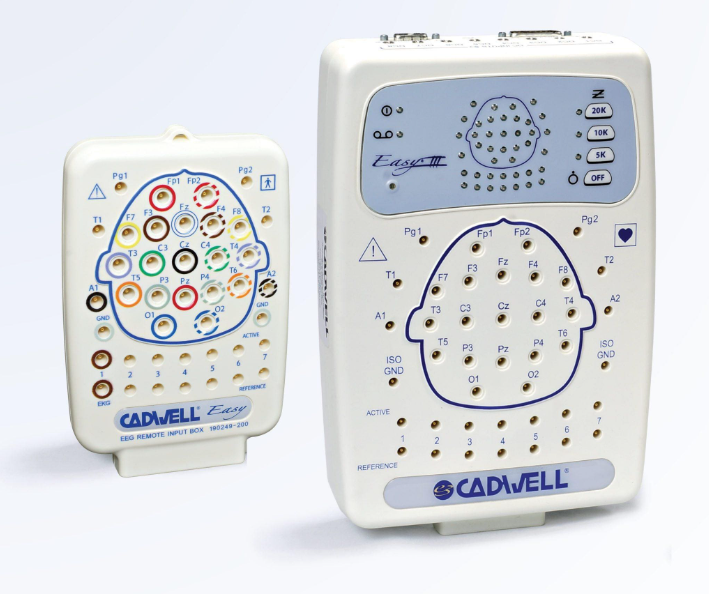
\includegraphics[
            width=\linewidth,
            height=5cm,
            keepaspectratio
        ]{Chapter2/Chapter2Figs/cadwell_modulos.png}

        \small (a) Módulos de adquisición EEG.
    \end{minipage}
    \hfill
    \begin{minipage}[c]{0.45\textwidth}
        \centering
        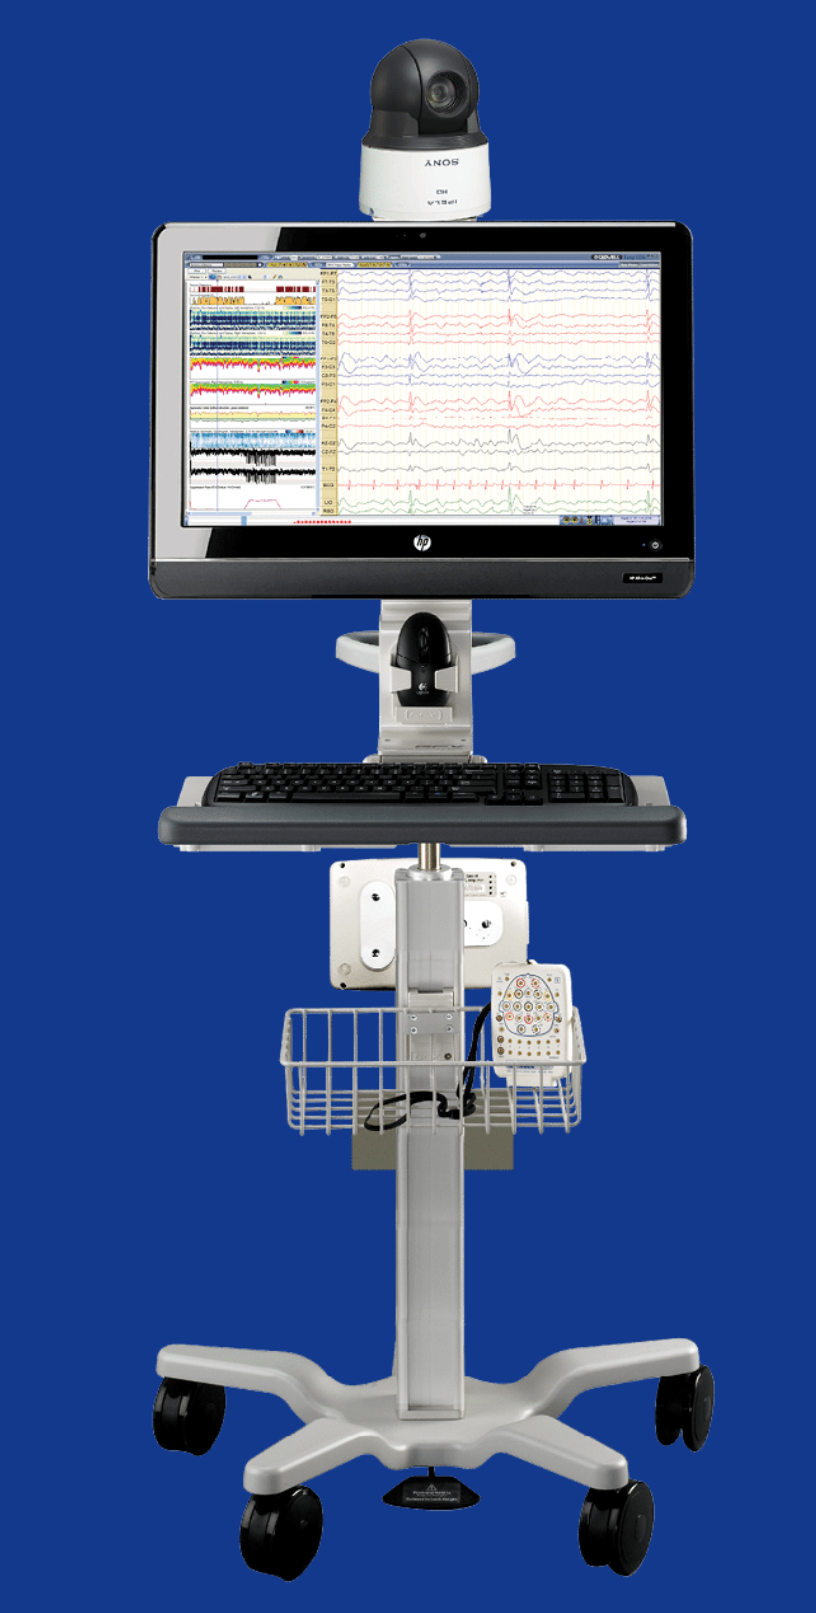
\includegraphics[
            width=\linewidth,
            height=5cm,
            keepaspectratio
        ]{Chapter2/Chapter2Figs/cadwell_estacion.png}

        \small (b) Estación de trabajo EEG.
    \end{minipage}

    \caption{Componentes del sistema Easy III EEG de Cadwell:
    (a) módulos de adquisición de señales y
    (b) estación de trabajo para visualización y revisión de EEG.
    Fuente: Cadwell Industries \citep{CadwellEasyIII}.}
    \label{fig:cadwell-easy-iii}
\end{figure}





\subsection{EEG Trend Software de Nihon Kohden}
\label{subsec:eeg-trend-nihon-kohden}

EEG Trend Software es una herramienta desarrollada por Nihon Kohden orientada
a la visualización y análisis de registros EEG, particularmente mediante el
uso de EEG cuantitativo y representaciones de tendencias. El \textit{software} permite observar cambios producidos a lo largo del tiempo y dispone de anotaciones
codificadas por colores y registros de eventos integrados como apoyo al
proceso de revisión \citep{NihonKohdenEEGTrend}.

La herramienta permite personalizar la disposición de las visualizaciones de
EEG y tendencias, así como comparar información correspondiente a diferentes
intervalos temporales. Los datos de registros prolongados pueden presentarse
mediante tendencias que condensan la información de varios días o incluso
semanas. Asimismo, el sistema dispone de herramientas de anotación y edición,
y contempla la utilización opcional de vídeo digital sincronizado para
contrastar las señales EEG con posibles artefactos observados durante el
registro \citep{NihonKohdenEEGTrend}.

Entre sus funciones de procesamiento se encuentra el análisis espectral de
las señales mediante la transformada rápida de Fourier (FFT). A partir de
este procesamiento, el \textit{software} puede presentar diferentes representaciones y parámetros, entre ellos arreglos espectrales de densidad (DSA), potencia, borde espectral y relaciones de potencia. También permite representar EEG integrado en amplitud (aEEG) y determinados parámetros relacionados con patrones de supresión de ráfagas \citep{NihonKohdenEEGTrend}.

EEG Trend Software incorpora además funciones orientadas a facilitar la
identificación de determinados eventos durante la revisión. De acuerdo con la documentación del fabricante, pueden utilizarse algoritmos opcionales de detección de crisis epilépticas en adultos y neonatos, los cuales señalan formas de onda que podrían corresponder a eventos electrográficos de interés para facilitar su posterior identificación y revisión. Asimismo, dispone de un mecanismo de detección de artefactos de electrodos que permite señalar tendencias que podrían estar influenciadas por dichos artefactos
\citep{NihonKohdenEEGTrend}.

Estas características muestran un enfoque en el que la visualización del EEG
puede complementarse mediante representaciones cuantitativas, análisis
espectral, tendencias y mecanismos automatizados de detección. La información
generada por estas herramientas puede facilitar la localización y revisión de
períodos de interés dentro de registros prolongados, manteniendo la señal EEG
como elemento fundamental para su interpretación.

\begin{figure}[htbp]
    \centering

    \begin{minipage}[c]{0.45\textwidth}
        \centering
        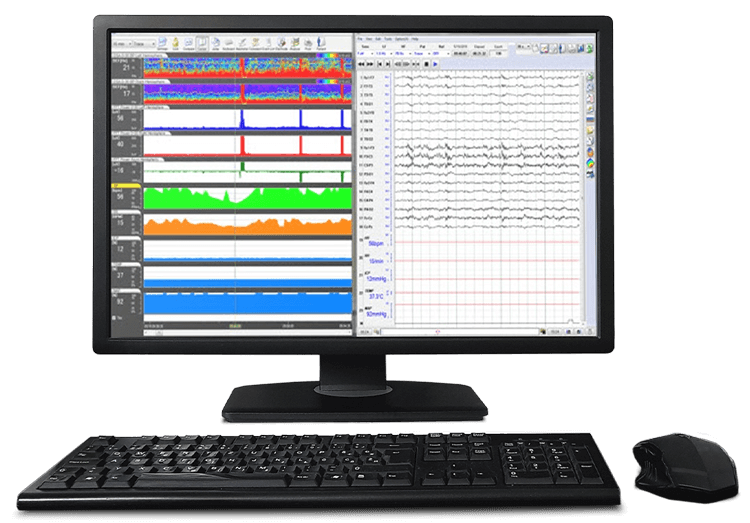
\includegraphics[
            width=\linewidth,
            height=5cm,
            keepaspectratio
        ]{Chapter2/Chapter2Figs/nihon_kohden_software.png}

        \small (a) Visualización de señales y tendencias EEG.
    \end{minipage}
    \hfill
    \begin{minipage}[c]{0.45\textwidth}
        \centering
        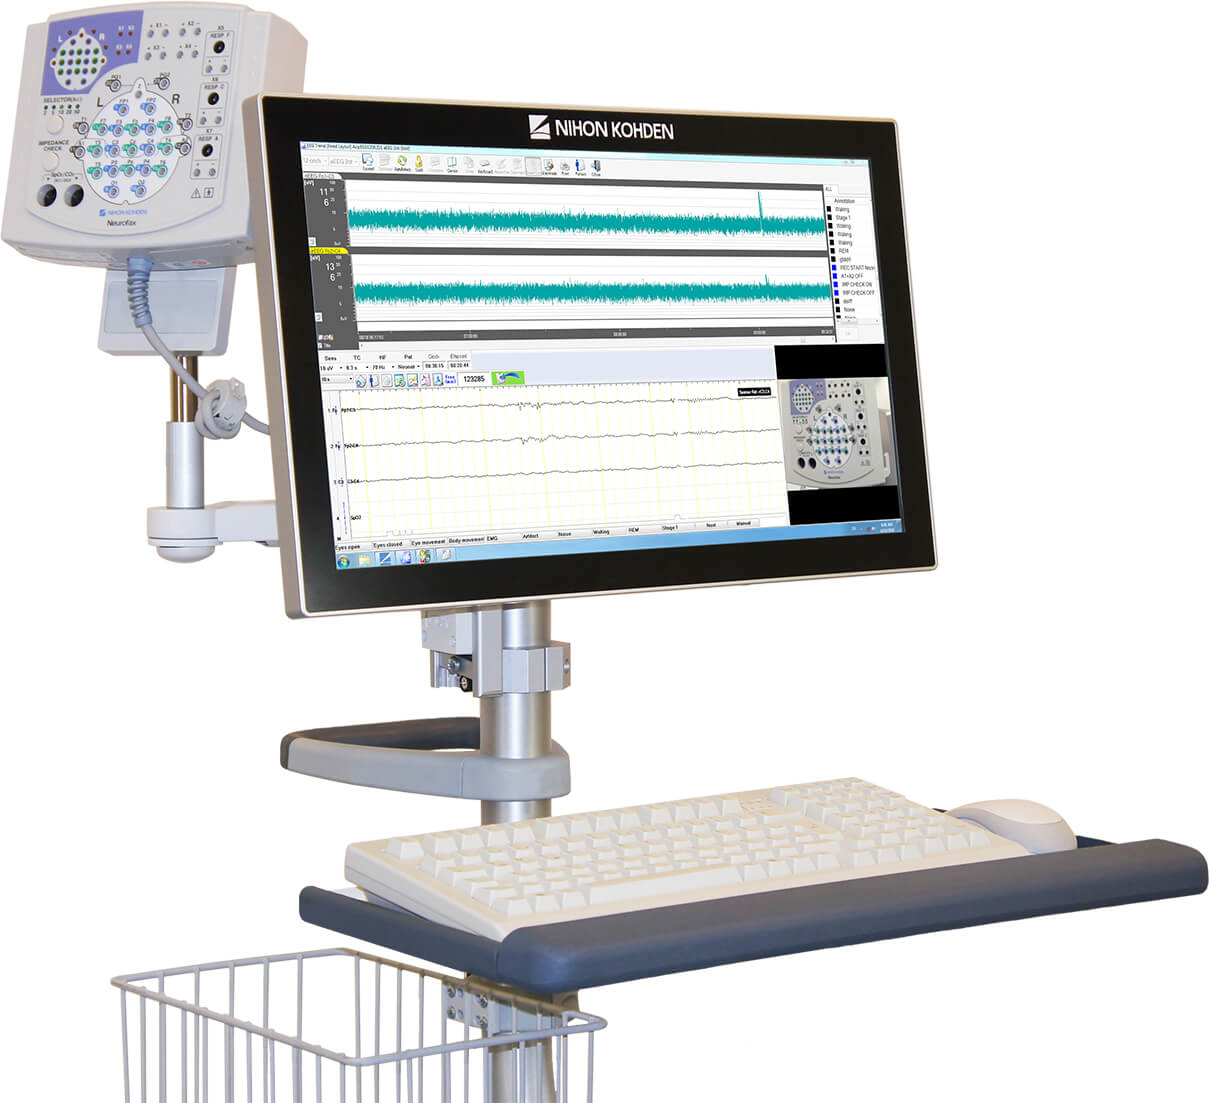
\includegraphics[
            width=\linewidth,
            height=5cm,
            keepaspectratio
        ]{Chapter2/Chapter2Figs/nihon_kohden_estacion.png}

        \small (b) Estación de trabajo EEG.
    \end{minipage}

    \caption{Herramientas de visualización y equipamiento EEG
    de Nihon Kohden: (a) interfaz de análisis de señales y
    tendencias y (b) estación de trabajo.
    Fuente: Nihon Kohden \citep{NihonKohdenEEGTrend}.}
    \label{fig:nihon-kohden-eeg-trend}
\end{figure}


\subsection{Plataformas web y herramientas relacionadas}
\label{subsec:plataformas-herramientas-eeg}

Además de los sistemas comerciales utilizados en entornos clínicos, existen
herramientas de código abierto destinadas al procesamiento, análisis y
visualización de señales EEG. Estas soluciones son utilizadas principalmente
en ámbitos de investigación y desarrollo, y proporcionan funcionalidades que
permiten trabajar con diferentes formatos de datos neurofisiológicos,
preprocesar señales, visualizar registros y aplicar distintos métodos de
análisis.

MNE-Python es una biblioteca de código abierto desarrollada en Python para el
procesamiento y análisis de datos neurofisiológicos, incluyendo señales EEG.
Esta biblioteca proporciona funcionalidades para la lectura de diferentes
formatos de datos, preprocesamiento, visualización de señales, análisis
tiempo--frecuencia, estimación de fuentes, conectividad, estadística y
aplicación de técnicas de aprendizaje automático
\citep{Gramfort2013MNE}.

Otra herramienta ampliamente utilizada es EEGLAB, un entorno de código abierto
desarrollado sobre MATLAB para el procesamiento de datos
electroencefalográficos. Permite importar y gestionar conjuntos de datos EEG,
visualizar señales y eventos, aplicar procedimientos de preprocesamiento y
realizar diferentes tipos de análisis. Su arquitectura admite además la
incorporación de extensiones mediante complementos desarrollados para tareas
específicas \citep{DelormeMakeig2004}.


Junto con estas herramientas, el desarrollo de tecnologías web ha permitido
la aparición de aplicaciones capaces de visualizar señales
electroencefalográficas mediante interfaces accesibles desde un navegador.
Entre los antecedentes se encuentra EpiCurrents, una herramienta orientada
a la visualización y revisión de señales neurofisiológicas en entornos web,
con funcionalidades para explorar registros electroencefalográficos
\citep{EpiCurrentsWebViewer}.
Este tipo de herramientas constituye un antecedente de la incorporación
de funcionalidades de revisión y análisis de señales EEG en entornos
interactivos basados en tecnologías web.


Las diferentes alternativas muestran que el análisis de EEG puede abordarse
mediante herramientas con propósitos y arquitecturas diversas. Mientras herramientas como MNE-Python y EEGLAB proporcionan recursos extensibles para el procesamiento y análisis de señales, las aplicaciones basadas en navegador
demuestran la posibilidad de ofrecer mecanismos interactivos de visualización
mediante tecnologías web. Estas características constituyen antecedentes
relevantes para el desarrollo de sistemas que integran gestión de información,
visualización de señales y herramientas de apoyo al análisis dentro de una
misma plataforma.


\section{Trabajos relacionados}
\label{sec:trabajos-relacionados}

El desarrollo de sistemas para el análisis de señales EEG ha sido abordado
desde diferentes perspectivas, incluyendo el procesamiento automatizado de
señales, la detección de patrones asociados con la epilepsia, la visualización
de registros electroencefalográficos y el desarrollo de herramientas de apoyo
para su revisión. Estos trabajos permiten identificar enfoques, tecnologías y
estrategias utilizadas previamente para resolver problemas relacionados con
el manejo y análisis de este tipo de información.

En esta sección se presentan antecedentes académicos sobre el análisis
automatizado y la visualización de señales EEG. Se consideran, en primer
lugar, investigaciones y desarrollos internacionales y, posteriormente,
trabajos realizados en la Facultad Politécnica de la Universidad Nacional
de Asunción (FP-UNA).

El análisis se centra en el propósito de cada trabajo, las técnicas y
herramientas empleadas y sus principales aportes al procesamiento, análisis
o visualización de señales EEG. Esta revisión permite identificar tendencias,
capacidades y limitaciones de las soluciones estudiadas.



\subsection{Antecedentes internacionales}
\label{subsec:antecedentes-internacionales}

Diversos trabajos internacionales han abordado el análisis de señales EEG
asociadas con la epilepsia mediante técnicas de procesamiento automatizado,
aprendizaje automático y plataformas informáticas orientadas a facilitar la
visualización y el análisis de los registros. Estos antecedentes permiten
observar la evolución desde métodos específicos de detección de crisis hasta
entornos web destinados al procesamiento y revisión colaborativa de señales
electrofisiológicas.

Shoeb et al. desarrollaron un método automatizado y específico para cada
paciente orientado a la detección del inicio de crisis epilépticas a partir
de EEG no invasivo. El método utilizó descomposición mediante \textit{wavelets} para obtener características relacionadas con la morfología y distribución
espacial de las señales, y posteriormente empleó una máquina de vectores de
soporte (SVM) para distinguir entre EEG correspondiente a crisis y actividad
no asociada con crisis. La evaluación se realizó sobre registros de 36
pacientes pediátricos con diferentes tipos de crisis, mostrando la
posibilidad de utilizar técnicas de aprendizaje automático para localizar
automáticamente eventos de interés dentro de registros EEG
\citep{Shoeb2004SeizureDetection}.

Desde una perspectiva orientada a la infraestructura y visualización,
Jayapandian et al. presentaron Cloudwave, una plataforma web destinada al
análisis y visualización de señales electrofisiológicas para investigación
clínica sobre epilepsia. La solución fue desarrollada en el marco del proyecto
Prevention and Risk Identification of SUDEP Mortality (PRISM) y utilizó
infraestructura de computación en la nube para proporcionar acceso a datos
compartidos. La plataforma permitió a investigadores de diferentes centros
buscar, consultar y visualizar eventos clínicos asociados con señales
anotadas, incluyendo patrones de crisis y otros eventos electrofisiológicos
\citep{Jayapandian2013Cloudwave}.


El desarrollo de Cloudwave constituye un antecedente relevante del
uso de tecnologías web para superar algunas limitaciones de las
aplicaciones instaladas de manera local. Su arquitectura fue planteada para
facilitar el acceso mediante navegador y el trabajo colaborativo sobre datos
electrofisiológicos compartidos, demostrando la posibilidad de trasladar
funciones de visualización y análisis de señales hacia una infraestructura
web \citep{Jayapandian2013Cloudwave}.

Posteriormente, Socrates et al. desarrollaron una aplicación web orientada al
procesamiento de señales de electroencefalografía estereotáxica (SEEG) para
el estudio de redes cerebrales relacionadas con la epilepsia. La plataforma
permite procesar señales SEEG de alta resolución y calcular diferentes
medidas de acoplamiento utilizadas para analizar conectividad funcional
cerebral mediante una interfaz gráfica. Los autores evaluaron además el
comportamiento de la aplicación frente al incremento del volumen de datos,
considerando la escalabilidad como parte de la solución
\citep{Socrates2019WebEEG}.

En conjunto, estos antecedentes muestran diferentes aproximaciones al apoyo
computacional del análisis de EEG en epilepsia. Algunos trabajos se concentran
en la identificación automatizada de crisis mediante técnicas de aprendizaje
automático, mientras que otros priorizan el acceso, procesamiento,
visualización y análisis colaborativo de señales mediante plataformas web.
Estos enfoques proporcionan referencias relevantes para sistemas que buscan
integrar procesamiento automatizado y herramientas de revisión de señales
dentro de un entorno informático accesible.

\subsection{Antecedentes desarrollados en la FP-UNA}
\label{subsec:antecedentes-fpuna}

En la Facultad Politécnica de la Universidad Nacional de Asunción se han
desarrollado investigaciones orientadas a la detección automatizada de crisis
epilépticas a partir de señales EEG mediante técnicas de aprendizaje
automático. Estos trabajos constituyen antecedentes nacionales relevantes
para el estudio de métodos de clasificación de señales electroencefalográficas.



Ayala-Britez, Frutos y Pinto-Roa estudiaron la detección de crisis epilépticas
a partir de señales EEG mediante características extraídas en el dominio
temporal y algoritmos clásicos de aprendizaje automático. El trabajo utilizó
registros de la base de datos CHB-MIT y analizó diferentes conjuntos de
características para distinguir segmentos correspondientes a crisis de aquellos
sin crisis. Entre los clasificadores considerados se incluyeron métodos como
máquinas de vectores de soporte (SVM), \textit{Random Forest} y
\textit{K-Nearest Neighbors} (KNN), evaluando su comportamiento
para la tarea de clasificación \citep{AyalaBritez2026SeizureDetection}.


Posteriormente, Lezcano, Ayala-Britez y Pinto-Roa ampliaron esta línea de
investigación mediante la incorporación de \textit{Gradient Boosting} para la detección automática de crisis epilépticas en señales EEG. El trabajo realizó una
comparación con modelos clásicos de aprendizaje automático y evaluó el
clasificador propuesto sobre características obtenidas de las señales. Los
resultados mostraron el potencial de los métodos de tipo \textit{ensemble}
para esta tarea de clasificación
\citep{Lezcano2026GradientBoosting}.

Estos antecedentes se centran principalmente en el procesamiento de
señales y en la construcción y evaluación de modelos capaces de distinguir
segmentos asociados con crisis epilépticas de aquellos sin crisis. Sus
aportes permiten reconocer posibilidades y limitaciones de los métodos
automatizados, así como la importancia de evaluar los modelos con datos
electroencefalográficos adecuados.



\section{Síntesis del estado del arte}
\label{sec:sintesis-estado-arte}

La revisión realizada a lo largo de este capítulo muestra que el análisis de
señales EEG en el contexto de la epilepsia involucra diferentes componentes
que abarcan desde la adquisición y representación de las señales hasta su
procesamiento, visualización e interpretación. La utilización de estándares
como EDF facilita el almacenamiento e intercambio de registros
electroencefalográficos, mientras que los montajes, filtros, parámetros de
visualización y representaciones tiempo--frecuencia proporcionan diferentes
formas de examinar la información contenida en estos registros.

En el ámbito clínico, la interpretación del EEG continúa requiriendo la
valoración del profesional especialista. Las técnicas de inteligencia
artificial y aprendizaje automático permiten complementar este proceso
mediante el análisis automatizado de las señales y la identificación de
segmentos que presentan determinados patrones de interés. Sin embargo, la
variabilidad de los registros, la presencia de artefactos y la posibilidad de
falsos positivos y falsos negativos hacen necesario que los resultados
generados automáticamente sean considerados como elementos de apoyo y
contrastados con la señal original y el contexto clínico.

Las herramientas revisadas muestran distintas aproximaciones al trabajo con
señales EEG. Sistemas especializados como Easy III EEG de Cadwell integran
funciones de adquisición, revisión y gestión de registros, mientras que EEG
Trend Software de Nihon Kohden incorpora representaciones cuantitativas,
tendencias y mecanismos automatizados de detección. Por otra parte,

herramientas de código abierto como MNE-Python y EEGLAB proporcionan
funcionalidades extensibles para el procesamiento y análisis de datos
neurofisiológicos. Los antecedentes basados en tecnologías web muestran además la posibilidad de trasladar funciones de acceso, procesamiento y visualización hacia entornos accesibles mediante navegador.

Los trabajos relacionados con la detección automatizada de crisis muestran,
a su vez, la aplicación de diferentes técnicas de aprendizaje automático
al procesamiento de señales EEG. En particular, los antecedentes
desarrollados en la FP-UNA contribuyen al conocimiento sobre la extracción
de características y la clasificación de segmentos electroencefalográficos,
complementando las investigaciones internacionales revisadas.



En conjunto, los antecedentes examinados evidencian que la gestión de
estudios, la visualización interactiva de señales, el procesamiento
automatizado y la elaboración de informes pueden abordarse mediante
herramientas especializadas o soluciones informáticas de distinto alcance.
Su integración plantea desafíos relacionados con la interoperabilidad,
la trazabilidad y la adecuada presentación de información para la revisión
por parte de profesionales clínicos.



En síntesis, el estado del arte permite identificar capacidades
complementarias entre los sistemas de adquisición y revisión de EEG,
las herramientas de análisis de señales, los modelos de aprendizaje
automático y las aplicaciones web. También pone de manifiesto la
necesidad de preservar la supervisión profesional, la integridad de
los registros y la trazabilidad de los resultados durante el análisis
electroencefalográfico.

\clearpage
\subsection{Comparación de herramientas y aporte de EpilexIA}
\label{subsec:comparacion-herramientas-epilexia}

A partir de las características descritas en los antecedentes, el
Cuadro~\ref{tab:comparacion-herramientas-eeg} presenta una comparación
sintética entre Easy III EEG de Cadwell, EEG Trend Software de Nihon
Kohden y la plataforma desarrollada en este trabajo. La comparación
considera el enfoque y las funciones documentadas de cada solución;
no constituye una evaluación experimental de su rendimiento clínico
ni presupone que las funciones no mencionadas estén ausentes.


\begin{table}[H]
\centering
\caption{Comparación de herramientas de análisis EEG y EpilexIA.}
\label{tab:comparacion-herramientas-eeg}
\scriptsize
\setlength{\tabcolsep}{3pt}
\renewcommand{\arraystretch}{1.10}

\begin{tabular}{|
>{\raggedright\arraybackslash}p{2.2cm}|
>{\raggedright\arraybackslash}p{2.75cm}|
>{\raggedright\arraybackslash}p{2.75cm}|
>{\raggedright\arraybackslash}p{3.25cm}|}
\hline
\textbf{Criterio} &
\textbf{Cadwell Easy III} &
\textbf{Nihon Kohden} &
\textbf{EpilexIA} \\
\hline

Enfoque &
Adquisición y revisión clínica de EEG. &
Análisis cuantitativo y tendencias EEG. &
Plataforma web para gestionar y revisar estudios EEG. \\
\hline

Visualización &
Señales, montajes y vídeo asociado. &
Señales, tendencias, espectrogramas y vídeo opcional. &
Señales EEG, filtros, sensibilidad, montajes y vídeo sincronizado. \\
\hline

Análisis automatizado &
No caracterizado en las fuentes revisadas. &
Algoritmos opcionales para señalar posibles eventos. &
Motor de IA integrado; validación integral pendiente. \\
\hline

Gestión clínica &
Gestión de registros e informes. &
Anotaciones y eventos durante la revisión. &
Gestión de pacientes, estudios, anomalías e informes por especialista. \\
\hline

Acceso &
Solución neurodiagnóstica especializada. &
Herramienta especializada de revisión EEG. &
Aplicación web accesible desde navegador, basada en componentes de código abierto. \\
\hline

\end{tabular}
\end{table}


Las capacidades de Easy III EEG y EEG Trend Software se resumen
según la documentación examinada \citep{CadwellEasyIII,CadwellEasyIIISpecifications,NihonKohdenEEGTrend}.
En este contexto, el aporte de EpilexIA consiste en reunir, en una
plataforma web, la gestión de pacientes y estudios, la visualización
interactiva de señales, el marcado de posibles anomalías y la elaboración
de informes médicos por especialista. Su arquitectura, basada en componentes de código abierto, favorece el mantenimiento, la evolución y la integración del sistema. La incorporación del análisis mediante IA representa una
capacidad prevista e implementada parcialmente en las verificaciones
documentadas, cuya eficacia diagnóstica y funcionamiento integral
requieren evaluación adicional. De esta manera, EpilexIA se plantea
como una herramienta complementaria de apoyo al profesional, sin
sustituir los sistemas de adquisición ni el juicio clínico especializado.

\clearpage